\documentclass[12pt,a4paper]{report}
\usepackage[pdftex]{color,graphicx}
%\usepackage[brazil]{babel}
\usepackage{amsmath}
\newcommand{\angstrom}{\textup{\AA}}
\usepackage{amsfonts}
\usepackage{amssymb}
\usepackage{graphicx}
\usepackage[utf8]{inputenc}
\usepackage[T1]{fontenc}
\usepackage[a4paper,left=2.0cm,right=2.0cm,top=2.0cm,bottom=2.0cm]{geometry}
\usepackage{fancyhdr}

\begin{document}
\fontsize{12pt}{17pt}\selectfont

\begin{titlepage}
\begin{center}

\includegraphics[width=0.2\textwidth]{./logo1.pdf}\\[0.2cm]
\textsc{UNIVERSIDADE FEDERAL DO PIAUÍ}\\[0.2cm]
\textsc{CENTRO DE CIÊNCIAS DA NATUREZA}\\[0.2cm]
\textsc{DEPARTAMENTO DE FÍSICA}\\[2.0cm]
{\textbf{Programa ICV/UFPI (2018/2019) – Relatório Parcial}}\\[1.0cm]
{\textbf{PLANO DE TRABALHO}}\\[0.4cm]
{\textbf{``Simulações computacional de cadeias lineares de carbono confinadas em nanotubos de carbono''}}\\[1.5cm]
{\textbf{PROJETO DE PESQUISA}}\\[0.4cm]
{\textbf{``ESTUDO COMPUTACIONAL DAS PROPRIEDADES VIBRACIONAIS E ELETRÔNICAS 
SISTEMAS HÍBRIDOS BASEADOS EM NANOTUBOS DE CARBONO''}}\\[2.0cm]

{Orientando: Antonio Lívio de Sousa Cruz}\\[1.0cm]
{Orientador: Acrisio Lins de Aguiar}\\[1.0cm]
{Teresina--PI, Fevereiro de 2019}
\end{center}
%Simulações computacionais de cadeias lineares de carbono confinadas em nanotubos de carbono.
\end{titlepage}
\setcounter{page}{2}

\chapter*{INTRODUÇÃO}
\paragraph{}
Desde que foram descobertos, os nanomateriais são estudados por conta da gama de utilizações, propriedades e tipos de estruturas encontrados relacionados aos mesmos. A partir de 1987, foram surgindo os primeiros trabalhos relacionados a nanotecnologia. Foi com o invento do 
microscopio de tunelamento (STM- Scanning Tunneling Microscope) que se tornou possivel a manipulacão de materiais nanométricos. Depois que o grafeno foi proposto por  Hanns-Peter Boehm, a pesquisa deste intrigante material e seus derivados vem crescendo exponensialmente pelo mundo, um exemplo é a dupla de pesquisadores Andre Geim e Konstantin Novoselov, da Universidade de Manchester, que receberam o Prêmio Nobel de Física de 2010.
\paragraph{}
A partir do grafeno são construidas outras estruturas, que dentre outras estão o grafino, o fulereno, e os nanotubos de carbono, que se diferenciam em suas diversas características estruturais, eletrônicas, térmicas e mais. Diante dessa imensa variedade, constatou-se que era necessário uma investigação a fundo para se conhecer toda a capacidade de cada uma dessas estruturas.
\paragraph{} Descobertos em $1991$ por S. Iijima, os nanotubos de carbono são atualmente um dos assuntos de destaque na nanociência e nanotecnologia, ultrapassando assim as barreiras da física, chegando a serem estudados nas áreas da biologia, ciência dos materiais, Farmácia, etc$[1]$. Desde o seu descobrimento, são estudadas suas propriedades térmicas, óticas, mecânicas e elétricas para que sejam de conhecimento as vastas possibilidades de utilização que possuem, segundo suas características. Assim, estas nanoestruturas podem ser utilizadas em diferentes tipos de materiais, como concreto, fibras, polímeros, sensores, dentre outros$[1]$. 
\paragraph{} Os CNTs(do inglês, \textit{carbon nanotubes}) podem ser descritos como o produto do enrolamento de uma folha de grafeno e podem ser classificados de duas maneiras. A primeira é dividida em dois grupos, no primeiro estam os nanotubos de uma única parede, ou SWNTs(do inglês, \textit{single wall nanotubes}), e no outro estão os nanotubos de múltiplas paredes, ou MWNTs(do inglês, \textit{multi wall nanotubes}), onde neste último grupo se destacam os DWNTs(do inglês, \textit{doble wall nanotubes}) e os TWNTs(do inglês, \textit{triple wall nanotubes})$[2]$. A segunda forma de classificação é feita pela forma com que a folha de grafeno é enrolada$[2]$, isso irá depender dos valores dos índices inteiros (n,m), do vetor quiral $\vec{C}_h$ e do vetor translacional $\vec{T}$. Então, se os índices são iguais (n,n) o nanotubo é do tipo \textit{armchair} (\textit{$\theta$} = $30^{o}$), se são arbitrários (n,m) é do tipo \textit{quiral}  e se tivermos m igual a zero (n,$0$) é do tipo \textit{zigzag} (\textit{$\theta$} = $0$), onde o ângulo $\theta$ é o ângulo quiral entre $\vec{C}_h$ e $\vec{T}$.
\paragraph{}  A simulação feita por computadores é um método utilizado para compreender as propriedades desse material, quando o experimento em si não se torna possível por conta de seu dificil acesso. Neste relatório, observamos por meio de simulações o comportamento de uma cadeia de carbono isolada por átomos de hidrogênio encapsulada por um nanotubo, dos tipos zigzag e armchair.



\chapter*{REVISÃO DA LITERATURA}
\paragraph{}
Tive como base a tese de mestrado de Marcelo Rodrigues dos Anjos para que pudesse começar os trabalhos com simulação da compressão de nanotubos, e para que pudesse ter um pouco mais de fundamento, extraí informações do artigo de Antonio Gomes de Souza Filho e Solange Binotto Fagan sobre funcionalização de nanotubos, onde os mesmos comentam sobre o processo de produção dos nanotubos, propriedades de sua estrutura e interações, dentre outros. No artigo de Marcelo Hawrylak Herbst, Maria Iaponeide Fernandes Macêdo e Ana Maria Rocco que fala da tecnologia relacionada ao nanotubos para que me acrescentasse sobre a utilização dos nanotubos na indústria e suas capacidades.


\chapter*{METODOLOGIA}
\subsection*{Produção do Nanotubo de Carbono}
\paragraph{}
Primeiramente, para que sejam feitos os estudos em um nanotubo de carbono, é de se imaginar que o primeiro passo para isso seja a produção de um. Tomando que este trabalho é baseado em simulações computacionais, o ferramental mais utilizado para isso é a linguagem de programação Fortran $90$, e,tendo isso em mãos ja podemos fazer a primeira parte da construção do nanotubo. Sendo o nanotubo um material derivado do grafeno, esta é a primeira estrutura a ser formada. Sabendo que a distância entre dois átomos de carbono($a_{c-c}$) é de $1,42 \angstrom$, definimos primeiro os vetores de base da rede triangular $\vec{a}_1$ e $\vec{a}_2$, separados por um ângulo de $60^{\circ}$, que farão a reprodução da rede como mostrado na figura $1a)$ abaixo. Mas, nao temos ainda a folha de grafeno que desejamos, visto que construimos a primeira rede triangular, para que fosse gerada a rede hexagonal foi feita uma reprodução de outra rede triangular por cima da primeira, mas deslocada a uma distância duas vezes maior que $a_{C-C}$ para o lado, assim, o resultado será uma rede hexagonal onde os átomos de carbono estarão igualmente espaçados.

\begin{figure} [!h]
\centering
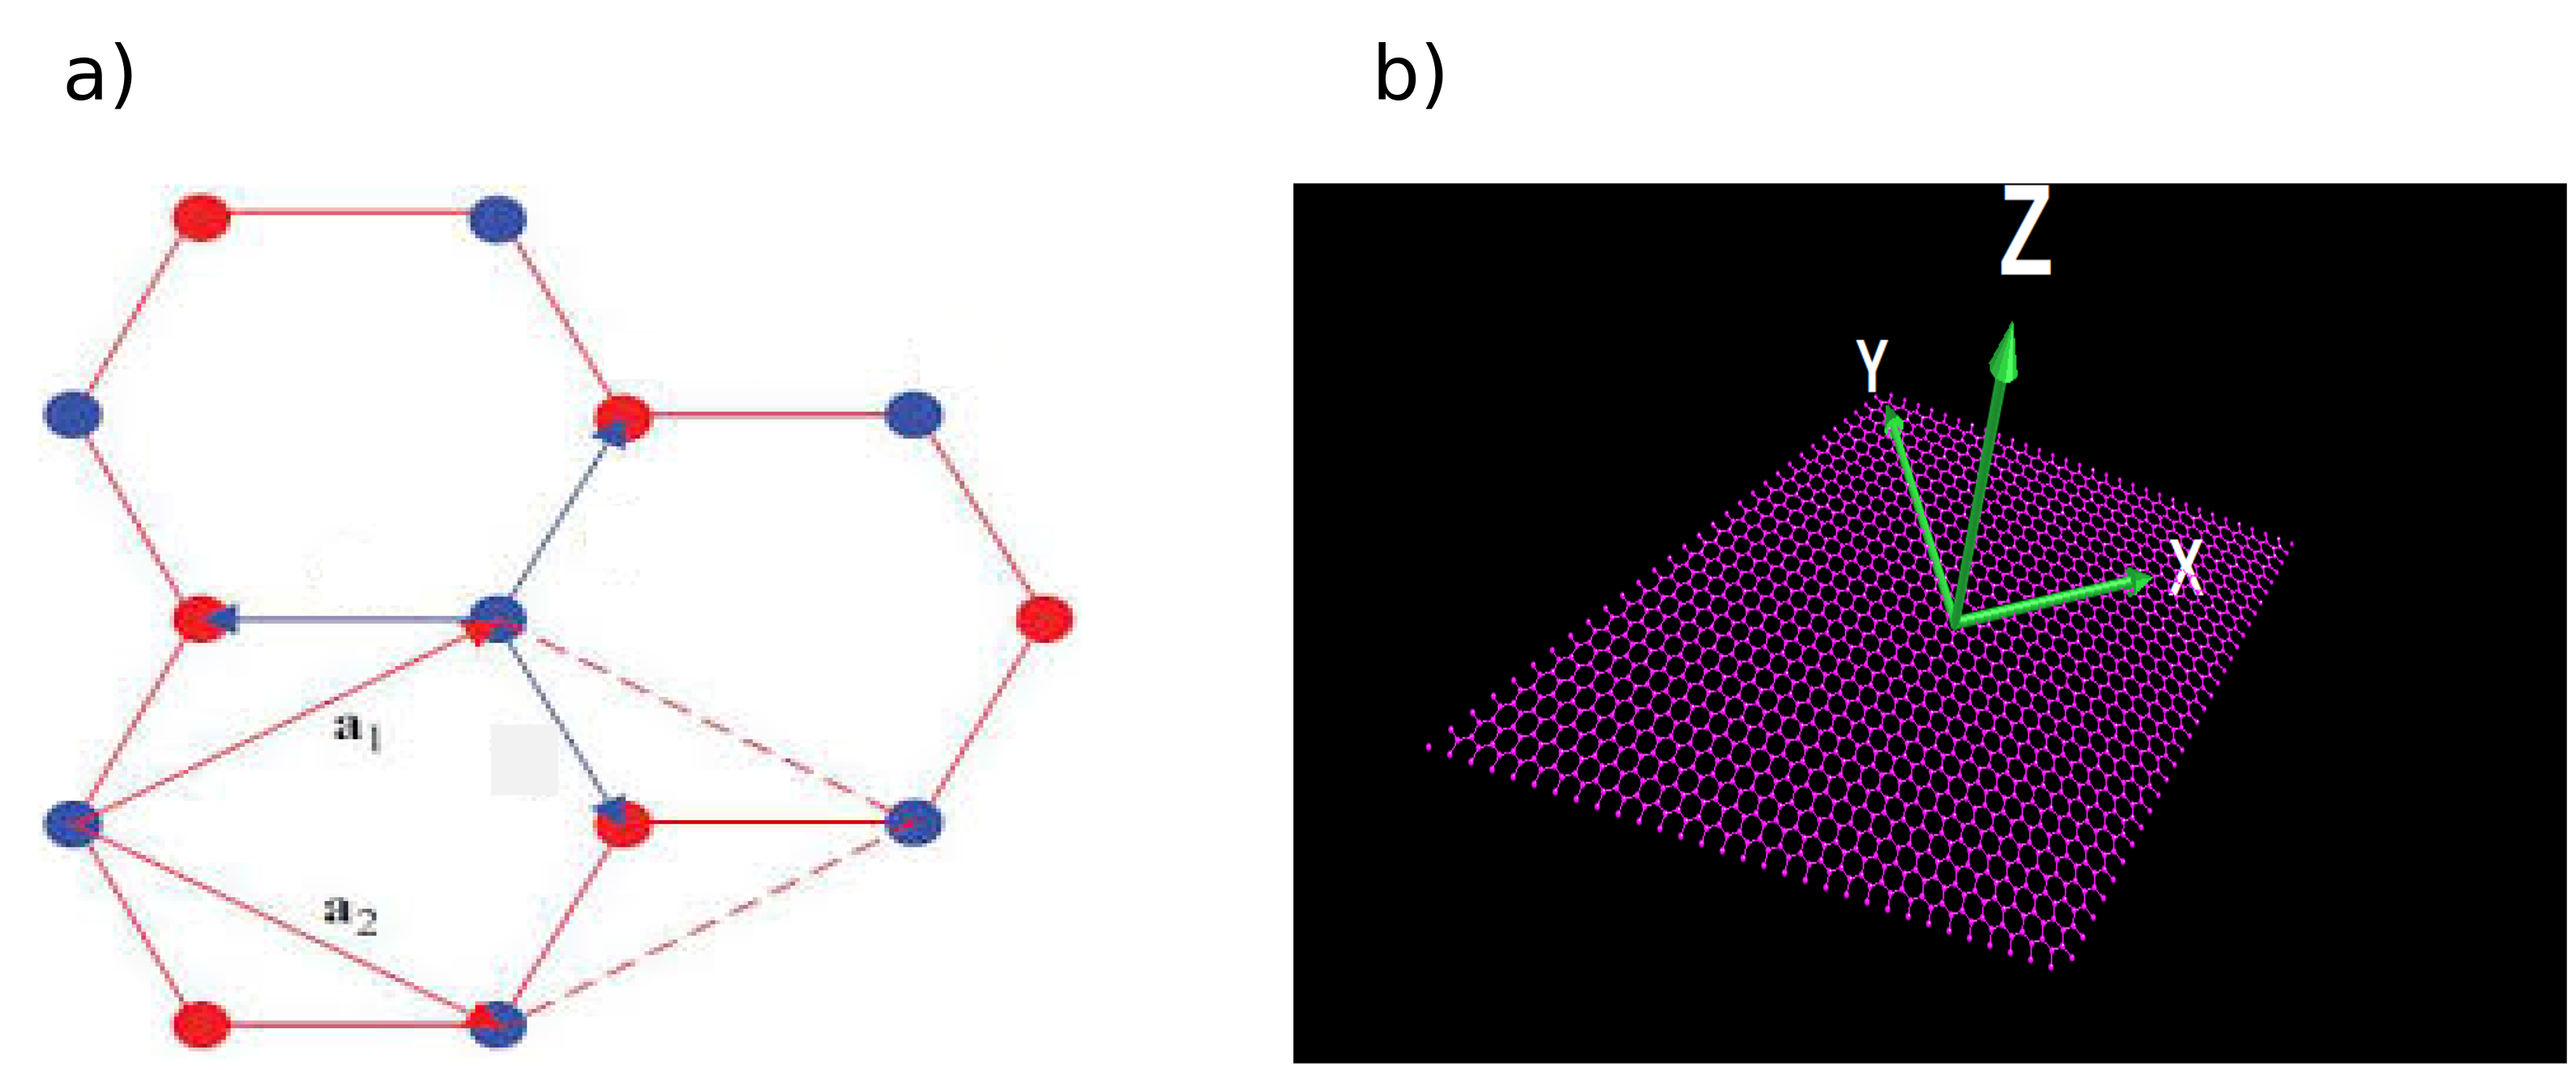
\includegraphics[scale=0.14]{print1.png}
\caption{a)Superposição de duas redes triangulares geradas pelos vetores de base $\vec{a}_1$ e $\vec{a}_2$, formando assim a rede hexagonal.b)Folha de grafeno construída no plano $(x,y)$.}
\end{figure}

\paragraph{}
Com nossa rede hexagonal feita, o próximo passo foi pensar em como tranfornar este material naquilo que queremos trabalhar é fazer um corte na mesma, como mostrado na figura $2$, onde tal corte é feito definindo dois vetores $\vec{R}_1=r_1\vec{a}_1+r_2\vec{a}_2$ e $\vec{R}_2=r_1\vec{a}_1+r_2\vec{a}_2+d\vec{i}$, os quais representam os dois diferentes átomos de carbono (em termos de simetria) da rede hexagonal e estão diretamente relacionados com os vetores $\vec{t}$ e $\vec{C}_h$, onde $r_1$ e $r_2$ variam de $0$ a $r_max$.

\begin{figure} [!h]
\centering
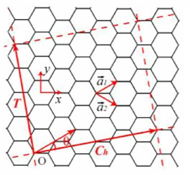
\includegraphics[scale=1.0]{corte2.png}
\caption{Corte feito em folha de grafeno para a produção do nanotubo de carbono.}
\end{figure}

\paragraph{}
Feito isso, fazemos uma mudança de coordenadas do nosso material simulado para coordenadas esféricas deixando-o enfim como o desejado. Temos como exemplo na figura $3$, onde temos três exemplos de nanotubos de quiralidades diferentes. 

\begin{figure} [!h]
\centering
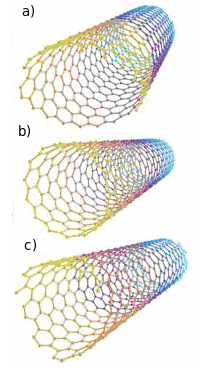
\includegraphics[scale=0.6]{cntclass.png}
\caption{a)Nanotubo de carbono do tipo armchair.b)Nanotubo de carbono do tipo zigzag.c)Nanotubo de carbono do tipo quiral.}
\end{figure}


\chapter*{RESULTADOS E DISCUSSÃO}
\paragraph{}
Tendo o processo para a produção do nanotubo sido feito, podemos seguir então com o objetivo que é enfim confinar uma cadeia de carbono, como a mostrada na figura $4$, em um nanotubo de carbono.

\begin{figure} [!h]
\centering
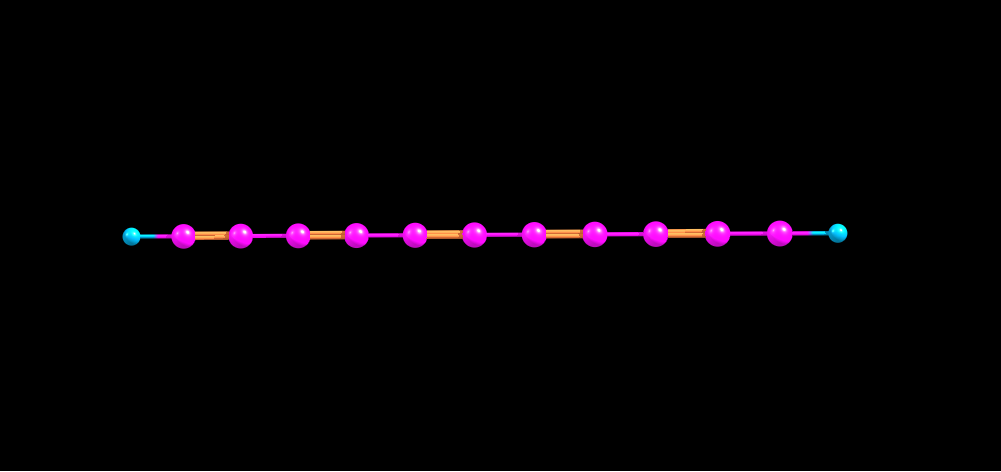
\includegraphics[scale=0.3]{chain.png}
\caption{Cadeia de átomos de carbono isolada por dois átomos de hidrogênio.}
\end{figure}

\paragraph{}
Isolamos assim a cadeia de átomos de carbono entre dois átomos de hidrogênio para que não pudesse ocorrer nenhum tipo de interação entre os átomos de carbono da cadeia com os da parede do nanotubo. Colocamo-la assim, no eixo central de um nanotubo para que pudesse se observar enfim as mudanças nas propriedades mecânicas do nanotubo, como pode-se ver nas figuras $5$ e $6$

\begin{figure} [!h]
\centering
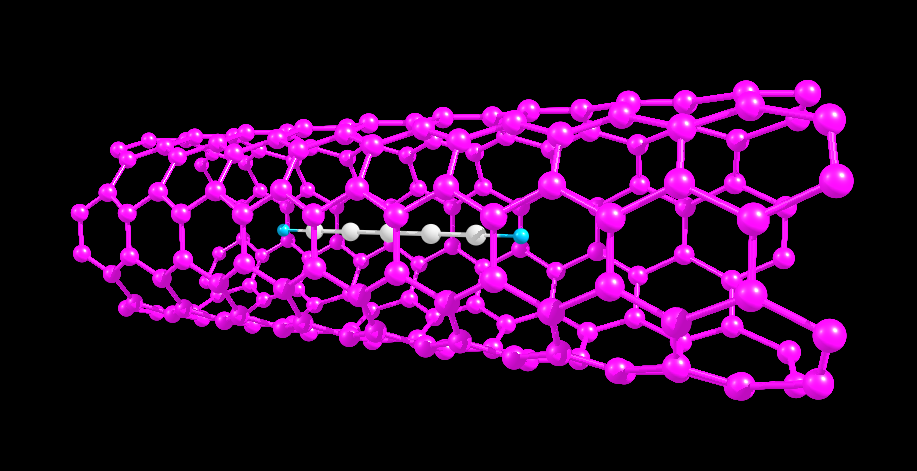
\includegraphics[scale=0.5]{cntc1.png}
\caption{Imagem lateral de um nanotubo $(5,5)$ com uma cadeia de 5 átomos de carbono confinada.}
\end{figure} 

\begin{figure} [!h]
\centering
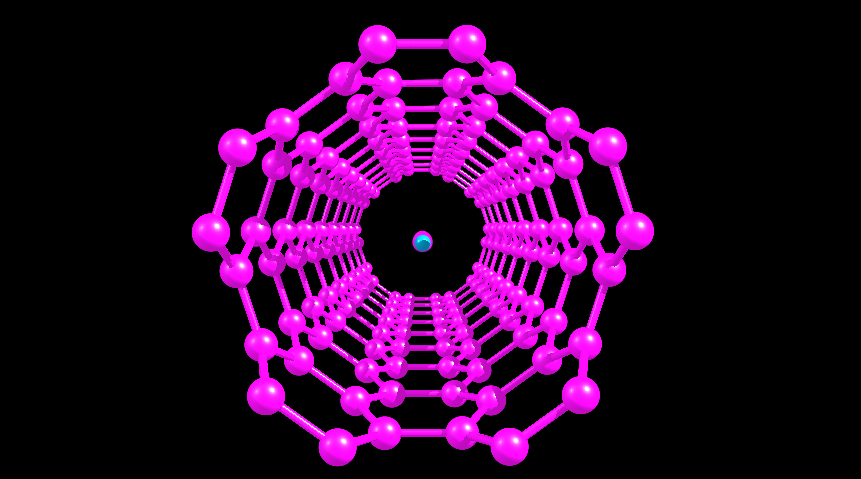
\includegraphics[scale=0.5]{cntc2.png}
\caption{Imagem frontal de um nanotubo $(5,5)$ com uma cadeia de 5 átomos de carbono confinada.}
\end{figure}

\paragraph{}
Na figura $5$, temos a cadeia com os átomos de carbono pintados de branco a fim de destacá-los enquanto na figura $6$, temos uma visão frontal da estrutura para que seja visível que a cadeia está no eixo central do nanotubo. Vale ressaltar que, nas imagens, os átomos pintados de azul são os átomos de hidrogênio.

\chapter*{CONCLUSÃO}
\paragraph{}
Podemos perceber que uma mudança estrutural é potencialmente capaz de causar mudanças nas propriedades da estrutura, no caso mecânicas, onde se espera que mude importantes valores como pressão de colapso, módulo de Bulk, e fração de volume, sendo essas as que provavelmente terão mudanças mais significativas.


\chapter*{REFERÊNCIAS}
\paragraph{}
[1]GOMES, A. de Souza Filho;FAGAN, Solange Binotto. Funcionalização de Nanotubos de Carbono, 2007;\\{0.5cm}

[2]DOS ANJOS, Marcelo Rodrigues.Estudo do Acoplamento em Nanotubos De Carbono e Duas e Três Camadas: Propriedades Mecânicas e Vibracionais.\\{0.5cm}

[3]HERBST, Marcelo Hawrylak; MACÊDO, Maria Iaponeide Fernandes; ROCCO, Ana Maria. Tecologia dos Nanotubos de Carbono:Tendências e Perspectivas de uma Área Multidisciplinar.



\end{document}
